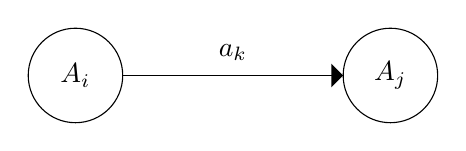
\begin{tikzpicture}[scale=0.2]
\tikzstyle{every node}+=[inner sep=0pt]
\draw [black] (0,0) circle (3);
\draw (0,0) node {$A_i$};
\draw [black] (20,0) circle (3);
\draw (20,0) node {$A_j$};
\draw [black] (3,0) -- (17,0);
\fill [black] (16.25,.75) -- (17,0) -- (16.25,-.75);
\draw (10,2) node [below] {$a_k$};
\end{tikzpicture}
